\chapter{Literature Review}
 
%%%%%%%%%%%%%%%%%%%%%%%%%%%%%%%%%%%%%%%%%%%%%%%%%%%%%%%%%%%%
%%%%%%%%%%%%%%%%%%%%  NEW SECTION   %%%%%%%%%%%%%%%%%%%%%%%%
%%%%%%%%%%%%%%%%%%%%%%%%%%%%%%%%%%%%%%%%%%%%%%%%%%%%%%%%%%%%
\setcounter{equation}{0}

%  START LITERATURE REVIEW FROM HERE.........

\section{Summary}

The sources explore Kolmogorov-Arnold Networks (KANs), a novel neural network architecture inspired by the Kolmogorov-Arnold representation theorem (KART). KANs present a potential alternative to the ubiquitous Multi-Layer Perceptrons (MLPs), offering advantages in accuracy and interpretability, particularly for scientific applications.
While MLPs utilize fixed activation functions on nodes ("neurons"), KANs implement learnable activation functions on edges ("weights"). This architectural shift replaces linear weight matrices with univariate functions, typically parameterized as B-spline curves. Nodes in a KAN perform simple summation, devoid of the non-linearity inherent in MLPs.

\begin{figure}[t]
    \centering
    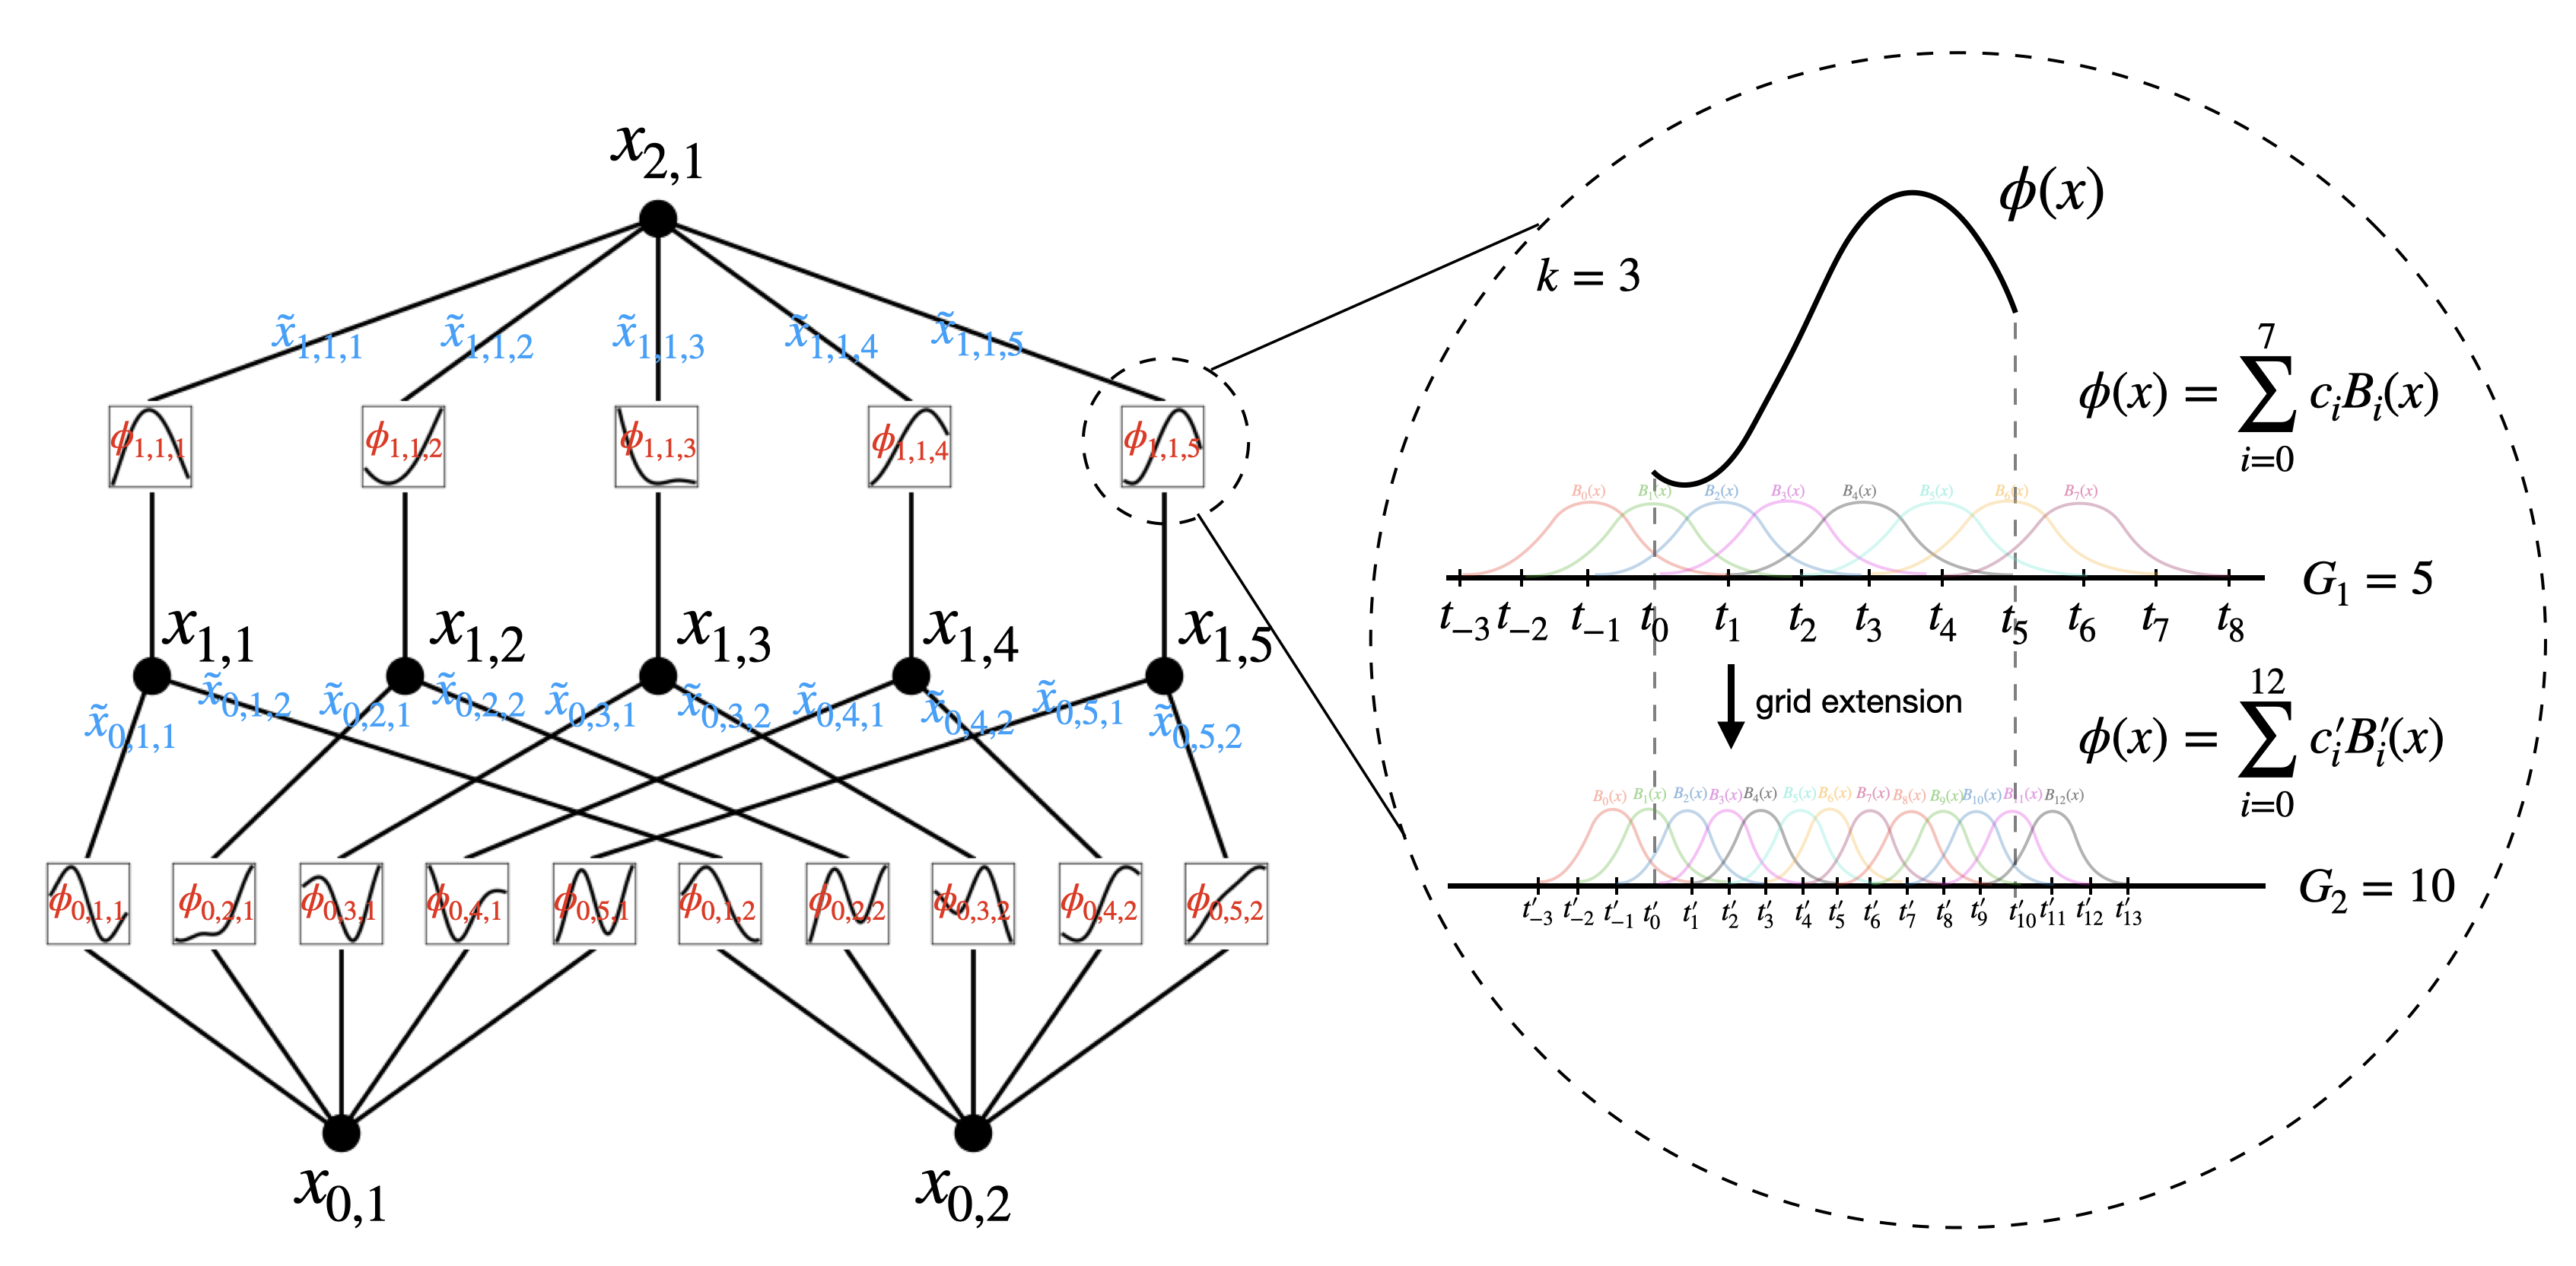
\includegraphics[width=0.9\linewidth]{Images/spline_notation.png}
    \caption{Left: Notations of activations that flow through the network. Right: an activation function is parameterized as a B-spline, which allows switching between coarse-grained and fine-grained grids.}
    \label{fig:spline-notation}
\end{figure}

The sources highlight two primary benefits of KANs:
\begin{itemize}
    \item Enhanced Accuracy and Scaling Laws: KANs, due to their ability to exploit compositional structures in data, exhibit promising scaling laws. This suggests they can achieve lower test errors with fewer parameters compared to MLPs, particularly for tasks involving symbolic formulas and special functions.
    \item Improved Interpretability: KANs leverage visually interpretable 1D activation functions, offering a more intuitive understanding of feature relationships compared to the opaque weight matrices in MLPs. Techniques like sparsification and pruning can further simplify KAN structures, facilitating the extraction of symbolic formulas and enhancing interpretability.
\end{itemize}

Balancing Interpretability and Scalability
A key consideration in KANs is the trade-off between interpretability and scalability. As KAN models grow larger, the sheer number of 1D functions, even if individually interpretable, can hinder overall understanding. This suggests that KANs might be most interpretable at smaller scales.
However, the sources propose various interpretability methods that can extend the interpretability of KANs to larger scales:

\begin{itemize}
    \item Symbolic Regression: Automatically converting trained activation functions into symbolic formulas.
    \item Modularity Discovery: Identifying groups of nodes and edges that form distinct functional modules within the network.
    \item Feature Attribution: Quantifying the importance of individual input features based on the activation patterns in the network.
\end{itemize}

KAN Implementation and Training
Effective implementation of KANs relies on careful consideration of training details:
\begin{itemize}
    \item Residual Activation Functions: A basis function, akin to residual connections, is added to each spline function. This improves trainability and mitigates vanishing gradients during backpropagation.
    \item Grid Points: B-splines are defined over a set of grid points, which determines the resolution of the function approximation. Increasing grid points generally improves accuracy but comes at the cost of increased model parameters.
\end{itemize}

    Applications in Scientific Discovery
    The sources demonstrate KANs' applicability to various scientific tasks, showcasing their ability to:
\begin{itemize}
    \item Uncover conserved quantities in physics.
    \item Identify phase transition boundaries in condensed matter physics.
    \item Reveal relationships in knot theory.
    \item Extract constitutive laws in materials science.
    \item Parameterize solutions to partial differential equations (PDEs).
\end{itemize}

Limitations and Future Research Directions
Despite their potential, KANs are still in the early stages of development, with areas for improvement:
\begin{itemize}
    \item Slow Training Speed: KANs, due to the computational complexity of B-spline operations, typically train much slower than MLPs. This poses a challenge for their application to large-scale datasets.
    \item Susceptibility to Overfitting: The smooth function approximation capability of B-splines may make KANs prone to overfitting, especially with noisy real-world data. Developing robust regularization techniques is crucial.
    \item Limited Generalizability: While KANs excel at representing specific function classes, their performance on broader machine learning tasks like computer vision, NLP, and audio processing requires further investigation. MLPs, with years of optimization, currently outperform KANs in these areas.
\end{itemize}

Future research on KANs should focus on:
\begin{itemize}
    \item Improving training efficiency through alternative activation functions, optimization methods, and hardware acceleration.
    \item Enhancing generalizability to diverse machine learning tasks beyond symbolic formula representation.
    \item Developing robust regularization techniques to mitigate overfitting.
    \item Exploring novel applications in science and engineering, leveraging interpretability and accuracy.
\end{itemize}


The emergence of KANs represents a significant step towards bridging the gap between connectionist AI and the symbolic nature of scientific knowledge. Their ability to decompose complex functions into interpretable units offers potential advantages for scientific discovery, knowledge extraction, and addressing the curse of dimensionality. While challenges remain in terms of training speed, overfitting, and generalizability, the unique properties of KANs make them a promising area for future research and development.
